This section is divided into three subsections. The first describes the fundamentals of finite field arithmetic. 
Then, the second subsection details the previous related works. And finally, in the last subsection, 
the contributions of this work are listed.

\subsection{Finite field arithmetic}

In this subsection, a quick review of the concepts related to Galois Field operators is made (for more details, refer to \cite{deschamps2009hardware}), 
focused on GF($2^m$). This field is an extension of GF(2), where the elements that make it up are zero and one. 
All finite fields have a unit element ($\alpha^0$), a zero element ($\alpha^{-\infty}$), a primitive element ($\alpha$), and at least one irreducible polynomial 
$p(x) = x^m + p_{m-1}x^{m-1} + ... + p_{1}x + p_{0}$. The primitive element $\alpha$ is the root of the irreducible polynomial and 
generates all the GF($2^m$) nonzero elements.


There are two ways to represent the elements in GF($2^m$): exponential and polynomial. 
In the exponential representation, the parts are defined as powers of $\alpha$, i.e.
\begin{equation}
 GF (2^m) = \{ 0, \alpha^0, \alpha^1, \alpha^2, ..., \alpha^{2m-2}  \}
 \label{eq:1}
\end{equation}
While the polynomial representation has the following form:
\begin{equation}
\begin{split}
 P(\alpha) = a_{m-1}\alpha^{m-1} + ... + a_{1}\alpha + a_{0};\\ 
 a_{i} \in GF(2), 0 \leq i \leq m-1
 \end{split}
 \label{eq:2}
\end{equation}


Polynomial representation is beneficial for doing arithmetic operations. %\cite{Jain1998}. 
The definitions of addition and multiplication of finite fields are given below.


\subsubsection{GF Addition}
Let's consider two elements of $a(x)$ and $a(x)$ (Eq. \ref{eq:3}), both belonging to the field $GF(2^m)$.
\begin{equation}
\begin{split}
 a(x) = a_{m-1}x^{m-1} + ... + a_{1}x + a_{0}\\
 b(x) = b_{m-1}x^{m-1} + ... + b_{1}x + b_{0}\\
 a_{i} \wedge b_{i} \in GF(2), 0 \leq i \leq m-1
 \end{split}
 \label{eq:3}
\end{equation}
The sum $s(x)$ (Eq. \ref{eq:4}) is directly the XOR operation of each of its coefficients. The result belongs to the same field.

\begin{equation}
 s(x) = (a_{m-1} \oplus b_{m-1})x^{m-1} + ... + (a_{0} \oplus b_{0})
 \label{eq:4}
\end{equation}


\subsubsection{GF Multiplication} \label{section:gf_mult}

There are different ways to multiply two polynomials in $GF(2^m)$. This paper focuses on two-step multiplication. As its name implies, 
this method separates multiplication into two steps: carry-less multiplication and polynomial reduction.


The first step is carry-less multiplication. The product $d(x)$ of the polynomials $a(x)$ and $b(x)$, is a polynomial of degree $2m-2$. 
This operation can be represented in matrix form as:

\begin{equation}
    \begin{pmatrix}
    d_{0} \\
    d_{1} \\
    \vdots \\
    d_{m-1} \\
    d_{m} \\
    d_{m+1} \\
    \vdots \\
    d_{2m-2} \\
    \end{pmatrix}
    =
    \begin{pmatrix}
        a_{0} & 0 & 0 & \cdots & 0 & 0 \\
        a_{1} & a_{0} & 0 & \cdots & 0 & 0 \\
        \vdots & \vdots & \vdots & \ddots & \vdots & \vdots \\
        a_{m-1} & a_{m-2} & a_{m-3} & \cdots & a_{1} & a_{0} \\
        0 & a_{m-1} & a_{m-2} & \cdots & a_{2} & a_{1} \\
        0 & 0 & a_{m-1} & \cdots & a_{3} & a_{2} \\
        \vdots & \vdots & \vdots & \ddots & \vdots & \vdots \\
        0 & 0 & 0 & \cdots & 0 & a_{m-1} 
    \end{pmatrix}
    \begin{pmatrix}
        b_{0} \\
        b_{1} \\
        b_{2} \\
        \vdots \\
        b_{m-2} \\
        b_{m-1} 
    \end{pmatrix}
\end{equation}

After the carry-less multiplication, the next step is the polynomial reduction based on an 
irreducible polynomial $f(x)$. In modular reduction $c(x) = d(x) mod f(x)$, the degree of $d(x)$ is 
reduced by the degree of the irreducible polynomial $f(x)$, resulting in a degree less than $m – 1$.
The matrix form of the polynomial reduction is showed in Equation \ref{eq:red}.


\begin{equation}\label{eq:red}
    \begin{pmatrix}
        c_{0} \\
        c_{1} \\
        \vdots \\
        c_{m-1} \\
    \end{pmatrix}
    =
    \begin{pmatrix}
        1 & 0 & \cdots & 0 & r_{0,0} & \cdots & r_{0,m-2} \\
        0 & 1 & \cdots & 0 & r_{1,0} & \cdots & r_{1,m-2} \\
        \vdots & \vdots & \ddots & \vdots & \vdots & \ddots & \vdots \\
        0 & 0 & \cdots & 1 & r_{m-1,0} & \cdots & r_{m-1,m-2} \\
    \end{pmatrix}
    \begin{pmatrix}
        d_{0} \\
        \vdots \\
        d_{m-1} \\
        d_{m} \\
        \vdots \\
        d_{2m-2} \\
    \end{pmatrix}
\end{equation}

The matrix $R$ in Equation \ref{eq:red} depends exclusively on the irreducible polynomial $f(x)$. 
The coefficients $r$ can be calculated as follows:

\begin{equation}
    r_{j,i}
    =
    \left\{\begin{matrix}
    f_{j};j=0,\hdots,m-1; i=0 \\ 
    r_{j-1,i-1}+r_{m-1,i-1}; j=0,\hdots,m-1;i=1,\hdots,m-2
\end{matrix}\right.
    \label{eq:red2}
\end{equation}


\subsection{Previous related works}

In this subsection, related works by other authors are presented.

The RISC-V community has proposed a scalar cryptographic extension \cite{zehrisc}. This instruction set 
accelerates various cryptographic algorithms, such as AES \cite{Marshall_Newell_Page_Saarinen_Wolf_2020}, SHA-256, SHA-512, SM3, and SM4. 
Although it achieves a considerable speedup, this proposal does not contemplate 
post-quantum (PQC) algorithms and error-correction codes. In this way, the instruction set is not flexible 
and cannot accelerate other algorithms or proprietary ciphers.


It can be observed that cryptography and error-correction codes share the same operations, such as 
bit manipulation (i.e. rotations, permutations, carry-less multiply) and finite field arithmetic.
These operations can be defined in the instruction set in order to accelerate a wider range of algorithms.
For example, a finite field $GF(q)$ ISA extension 
was proposed in Alkim's \cite{Alkim_Evkan_Lahr_Niederhagen_Petri_2020} work to accelerate lattice-based PQC 
cryptography (Kyber, NewHope). The same can be done for the $GF(2^m)$ fields to speed up code-based PQC, 
error-correction codes, and basic operations of classical cryptography \cite{10.1145/944645.944659}.

\subsection{Contributions}

\begin{figure*}[tp]
    \centering
    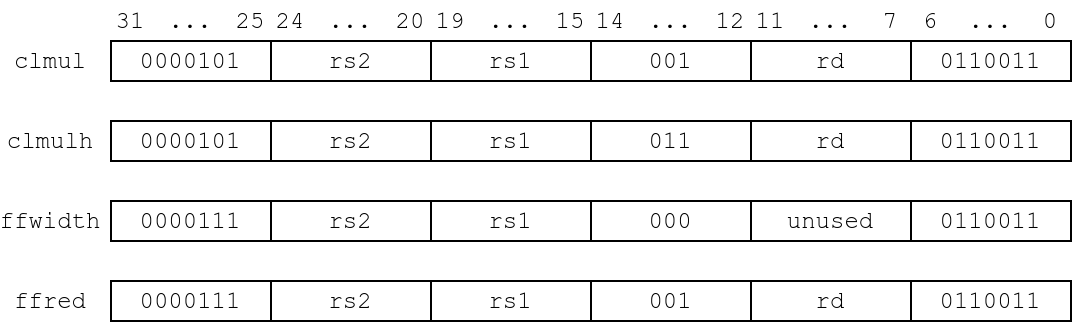
\includegraphics[width=0.8\linewidth]{img/instr.png}
    \caption{The instruction format for the custom Galois field arithmetic instructions.}
    \Description{The instruction format for the custom Galois field arithmetic instructions.}
    \label{fig:instr}
\end{figure*}

%With the rise of Edge Computing, IoT end-nodes \cite{8123913} and satellites \cite{8945402} must process different communication and data encryption protocols, 
%either standard protocols or proprietary. Therefore, some flexibility is required for this kind of processor.
%As $GF(2^m) $ arithmetic is presented in most communication systems, an extension of the RISC-V ISA is proposed in this work. 

The contribution of this work is an solution between the RISC-V base ISA and the scalar cryptographic K extension \cite{zehrisc}, resulting in an 
intermediate performance between the two. However, with greater flexibility in the protocols that it can process. 

The RISC-V ISA K extension can accelerate SHA2, AES, SM3, and SM4 using dedicated instructions, and they plan to support more algorithms 
in the future (Aria, Camelia, NIST LWC, and PQC algorithms). As this extension implements dedicated hardware for each algorithm, the execution time is faster, but the area is much larger than that of our proposal.

Our proposed ISA extension is capable of processing the following algorithms:

\begin{itemize}
    \item Non-binary error-correction codes (i.e., Non-binary low density parity check (LDPC), BCH, RS codes, \dots)
    \item Pre-quantum cryptography (i.e., AES, Elliptic Curve, \dots)
    \item PQC cryptography (i.e., McEliece, Rainbow, HQC, \dots)
\end{itemize}


